In this chapter, some related work of this thesis is presented. The first section gives the classification of elasticity mechanisms as proposed by \cite{galante2012survey} \cite{dawoud2013scalability} \cite{lorido2012auto}. In the second section the state of the art techniques in autoscaling such as time series forecasting and threshold based mechanism which is investigated and applied in this thesis are presented. Finally an analysis and evaluation of the work done on the state of the art simulation methods in cloud computing research is presented.

\section{Classification of elasticity mechanism}
\label{sec:Classification of elasticity mechanism}
Classification of various autoscaling techniques based on the elasticity mechanism will help in classifying state of the art autoscaling techniques. This section provides a comprehensive study about various elasticity mechanism available today. In the first part of this section, classification of various elasticity mechanism  is presented which is proposed by \cite{galante2012survey} \cite{dawoud2013scalability} \cite{lorido2012auto}. The classification created here for the purpose for this thesis is based upon the works of \cite{galante2012survey} \cite{dawoud2013scalability} \cite{lorido2012auto}. Galante et al.\cite{galante2012survey} purposed a classification of elasticity mechanism based on four characteristics:
\begin{enumerate}
  \item Scope
  \item Policy
  \item Purpose
  \item Method
\end{enumerate}
Classification purposed by the authors can be illustrated in Figure~\ref{figure:elasticclassification}. This classification is based on various studies done on academics research and cloud service providers recommendation. The classification proposed by Galante et al.\cite{galante2012survey}, calls Horizontal scaling as replication of virtual machines, and Vertical scaling as re-dimensioning of virtual machines.

\begin{figure}[h]
  \begin{center}
    \begin{forest}
   for tree={grow=0,parent anchor=east, child anchor=west, edge path={\noexpand\path[\forestoption{edge}] (\forestOve{\forestove{@parent}}{name}.parent anchor)-- +(0:2mm)|-(\forestove{name}.child anchor)\forestoption{edge label};}}
  [Elasticity
    [Scope
        [Infrastructure]
        [Application]
    ]
    [Policy
        [Manual]
        [Automatic
            [Reactive]
            [Proactive]
        ]
    ]
    [Purpose
        [Performance]
        [Increase Elasticity]
        [Cost]
        [Energy]
    ]
    [Method
        [Horizontal]
        [Vertical]
        [Migration]
    ]
  ]
  \end{forest}
    \caption{Classification of Elasticity (From \cite{galante2012survey})}
    \label{figure:elasticclassification}
  \end{center}
\end{figure}

\section{State of Art}
\label{sec:State of Art}
In recent years, lots of state-of-the-art\cite{lorido2012auto} techniques for horizontal scalability have been successfully developed in research institutes and industries. These developed scalability solutions have turned out to be very helpful and valuable tools in scientific researches as well as commercial products. In this section diverse related work is reviewed in order to present the state of the art auto scaling techniques in clouds.

\subsection{Threshold Based Rules}
\label{sub:Threshold Based Rules}
Galante at el.\cite{galante2012survey} defines the threshold or rule based mechanism for horizontal scaling as a Rule-Condition-Action mechanism. Rules consists of set of conditions upon meeting these conditions appropriate scaling actions are trigged. Every condition consists of performance metric from the system which is compared against a threshold. The information about the performance metric values are provided by the infrastructure monitoring system\cite{lorido2012auto}. Each threshold is defined by the user and its composed of two parameters: an upper threshold and a lower threshold for each performance metric\cite{lorido2012auto}. The scaling action will scale the resource based on the  type of scaling. For horizontal scaling, the user will define fixed number VM instances to create or destroy, but for vertical scaling user will define the amount to resources of a particular resource type to be added or removed to the VM. An example for a threshold based rule is: add two instance when the number of user sessions exceeds  100 user sessions per instance\cite{lorido2012auto}.
Amazon AWS offers horizontal scaling mechanism called Auto Scaling as part of its EC2 service\cite{AmazonAutoScale}. The solution is based on a concept called Auto Scaling Groups(AGS)\cite{AmazonAutoScale}. AGS consists of a set of instances that can be used by an application. Amazon Auto Scaling mechanism uses an automatic-reactive approach\cite{galante2012survey}. Foreach AGS, rules are defined to add or release predefined number of instances\cite{AmazonAutoScale}.
\\
RightScale\cite{Rightscale}, a popular cloud management solution for managing cloud infrastructure across multiple IaaS providers, provides horizontal autoscaling mechanism which uses a simple democratic voting to scale up or down\cite{galante2012survey}. Running VM instance participate in the process of voting and scaling action is taken based on majority of votes. After each scaling action a cooldown time is introduced where in no scaling action will be taken\cite{lorido2012auto}. This cooldown time is provided to prevents the algorithm from continually allocating resources as new instances boot\cite{kupferman2009scaling}. Rightscaling algorithm is highly dependent on user-defined values for threshold and cooldown time, if these values are not optimally tuned it can lead to rapid starting and termination of machines due to rapid spikes in workload. Kupferman et al.\cite{kupferman2009scaling} extends the RightScale algorithm with a concept called smart kill. The authors\cite{kupferman2009scaling} considers the fact that machines are charged by cloud service providers in hourly basis. This approach does not terminate the instances even if the load is low and the instance is not required, because the instance will be paid for entire hour, and there no reason to terminate the instance before the finish of instance hour\cite{kupferman2009scaling}.
\subsection{Reinforcement Learning}
\label{sub:Reinforcement Learning}
Reinforcement learning is an automatic decision making process which is applicable for autoscaling mechanism\cite{lorido2012auto}. Reinforcement learning\cite{Reinforced} is defined as an automated approach to goal oriented learning and decision making. Learning is done through directed interaction between agent and its environment. Reinforced learning process can be illustrated from the Figure~\ref{figure:reinforced}. Agent is the  decision-maker that learns from its experience to make best action to execute for each state of the environment and always try to maximize the reward\cite{Reinforced}. In terms of autoscaling problem, the autoscale algorithm is the agent that interact with the application environment. This will decide whether to add or remove (actions) VM instances to the system depending on the workload, performance or other set of metic(state). This process always tries to minimize the values like response time, cost (reward) etc.
\begin{figure}[h]
  \begin{center}
    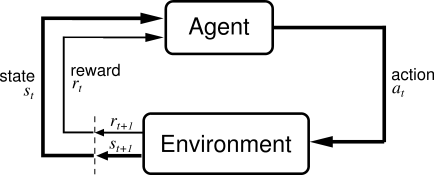
\includegraphics[scale=0.9]{reinforced.png}
    \caption{The agent-environment interaction in reinforcement learning (From\cite{Reinforced})}
    \label{figure:reinforced}
  \end{center}
\end{figure}
Yazdanov et al.\cite{yazdanov2013vscaler} proposes a concept called VScaler, which is a framework implementing autonomic resource allocation using reinforcement learning. Here authors model the  states as number of VM's running, actions are amount of VM's which can be added, removed or maintained\cite{yazdanov2013vscaler}, and utilization of the VM's as reward function. In works of\cite{barrett2013applying},\cite{dutreilh2011using},\cite{rao2009vconf} reward function is studied in perspective of cost of VM machines and  SLO violations.
\\
Although reinforcement learning methods for autoscaling look promising,\cite{lorido2012auto} points out several problems:
\begin{itemize}
  \item Curse of dimensionality problem\cite{yazdanov2013vscaler}: The size of the state space grows  exponentially with each added new state variable. Yazdanov\cite{yazdanov2013vscaler} estimates there will be 10240 states if VM's with two resource parameters, 10 different values for each parameter and 10 actions for every state.
  \item Large learning time \& bad initial performance: Agent in reinforcement learning approach learns about its environment by visiting each state-action pair. Therefore learning process time depends on the size of state-action space. Large initial learning process leads poor initial performance of the reinforcement algorithm.
\end{itemize}
In order to improve the bad performance Yazdanov\cite{yazdanov2013vscaler} proposed a reinforcement learning model with parallel learners to speed up the agent learning process.
\subsection{Time-series Analysis}
\label{sub:Time-series Analysis}
Time series analysis uses historical data to predict future workloads. Time series are used in many domain such as engineering, finance, economics and bioinformatics, to represent changes in the system over time. Time series analysis and forecasting methods are generally used in proactive autoscaling mechanisms. In 2012 Herbst\cite{herbst2012workload} published his diploma thesis from University of Wuerzburg on workload classification and forecasting. This work presents a detailed survey of various methods in time series analysis and forecasting. The author made a detailed survey and grouping of various time series and  forecasting based on their strengths and weakness. Based on this comparative study a dynamic approach know as WorkloadClassificationAndForecasting (WCF)\cite{herbst2012workload} is developed. WCF\cite{herbst2012workload} has capability to dynamically create time series model for a given time series data. The author has implements WCF as Java based software\footnote{\url{https://github.com/NikolasHerbst/WCF}} which is used extensively in research community. Here\cite{herbst2012workload} it also proves from experimental setup that the effect of workload forecasting in proactive resource provisioning can avoid 52\% to 70\% SLA violations. A subset of the survey on time series forecasting published by the authors\cite{herbst2012workload} is presented in the Table~\ref{table:tssurvey}.
\\
In work done by Roy et al.\cite{roy2011efficient}, authors proposed autoscaling by static threshold based method in combination with workload forecasting. Here the authors have used second order autoregressive moving average method (ARMA) for workload forecasting and combines with response time and server utilization as autoscaling thresholds. Further, Islam et al.\cite{islam2012empirical}, proposed a proactive prediction based autoscaling strategies using Neural Network and Linear Regression.
\begin{flushleft}
  \begin{table}
    \begin{tabular}{ | L{2cm} | L{2cm} | L{2cm} | L{2cm} | L{2cm} | L{2cm} |}
      \hline
      Name & Forecast horizon & Historical data & Strengths & Weakness & Suitable for use case \\ \hline
      Naive forecasting  & 1-2 points & Single previous observation & No historical data required & No use in proactive autoscaling as the prediction horizon is too small & Constant arrival rate \\ \hline
      Moving average (MA) & 1-2 points & Two consecutive observations & Simplicity & Sensitivity to trends and seasonal components & Constant arrival rate with low white noise \\ \hline
      ARMA & less than 5 points & Small number of historical data & Trend estimation is possible and has fast forecast performance & No season component in included model, only positive time series & Time series with some noise and trend\\ \hline
      ARIMA\cite{box2015time} & more than 5points & At least 3 periods in time series data & Capturing noise, trend and season component & Complex modeling & Times series with seasonal component and moderate noise level\\ \hline
    \end{tabular}
    \caption{Table of Forecast Strategies and their Properties (From\cite{herbst2012workload})}
    \label{table:tssurvey}
\end{table}
\end{flushleft}

\subsection{Combined Approach}
\label{sub:Combined Approach}
In the recent years, the above mentioned scaling mechanism has be combined and studied to develop an efficient proactive scaling mechanisms. These methods are widely researched and published by Roy et al.\cite{roy2011efficient}, Sharma\cite{sharma2011cost}, AzureWatch\cite{Azurewatch}, Gong\cite{gong2010press}, Nguyen\cite{nguyen2013agile}. Roy et al.\cite{roy2011efficient} in their paper developed a proactive look-ahead technique for workload forecasting using ARMA time series forecasting strategy working in combination with threshold rules defined on utilization of each VM (taking mean value of utilization). The authors objective was to minimize resource usage, satisfy the application QoS and keep operational cost low\cite{galante2012survey}.
\\
PRESS was developed by Gong\cite{gong2010press} which uses signal processing techniques to identify patterns in the workloads. These identified patterns are then used to predict future workload. PRESS fall back to statistical state machine based approach if there were no pattern emerged from the historical workload. This approach helps application maintain SLA guarantees with minimum resource allocation. Nguyen\cite{nguyen2013agile} developed a concept called AGILE, which is a proactive scaling mechanism uses wavelet transformation for workload forecasting\cite{nguyen2013agile}. AGILE uses a concept called resource pressure which is a ratio of resource usage for scaling the resources.
\\
AppElastic algorithm developed in this thesis tries to extent the concept of\cite{roy2011efficient}. In contrast to  Roy et al.\cite{roy2011efficient}, AppElastic algorithm uses ARIMA forecasting. ARIMA forecasting models are generally used to predict future workload point for more than five mins (as shown in the Table~\ref{table:tssurvey}). It also differs from \cite{roy2011efficient} by using number of active sessions per VM instances as threshold for scaling.

\section{Cloud Simulation Methods}
\label{sec:Cloud Simulation Methods}
Evaluating the effectiveness of a autoscaling algorithm is often realized over the time spent in production system operating under hight workloads\cite{AlexanderSim}. When working with production system workload trace, which generally spans over multiple months, empirical evaluation of autoscaling algorithms on real-time production system workload trace is infeasible. To address this challenge, academic community has put forward several approaches to simulate the autoscaling algorithm evaluation.
\\
Through these simulation approach systems can be evaluated from two perspectives one from IaaS cloud perspective and other from the application perspective. Pucher\cite{AlexanderSim} in his blog post summarizes a list of popular simulation software widely used by the research community. Pucher\cite{AlexanderSim} classifies simulation software developed in academia into Infrastructure Simulators and Application-perspective cloud simulators. A survey of these simulators presented by Pucher\cite{AlexanderSim} is presented below.
\subsection{Infrastructure Simulators}
\label{sub:Infrastructure Simulators}
Infrastructure simulators are used to simulate cloud computing infrastructure and services. It is widely used among the cloud computing research fields such as fault-tolerance, scalable computing such as MapReduce\cite{dean2008mapreduce} etc. Two widely used infrastructure simulators are listed below:
\begin{itemize}
  \item Cloudsim\cite{calheiros2011cloudsim}: Cloudsim is used for modeling, simulation, and experimentation of emerging Cloud computing infrastructures and application services. Cloudsim provides modeling and simulation features for large scale Cloud computing data centers\cite{Cloudsim}, virtualized server hosts\cite{Cloudsim}, data center network topologies and message-passing applications\cite{Cloudsim} and much more.
  \item GreenCloud\cite{kliazovich2012greencloud}: GreenCloud is used to develop simulation of monitoring of resource, resource allocation, workload scheduling and network infrastructures\cite{Greencloud}. GreenCloud simulate cloud computing resources such as CPU, memory, storage and networking resources. It also supports energy models of all resource types and provides a GUI for its users. GreenCloud is widely used among the research communities studying energy aware cloud computing systems.
\end{itemize}

\subsection{Cloud Hosted Application Perspective Simulators}
\label{sub:Cloud Hosted Application Perspective Simulators}
Cloud hosted application simulators are designed to simulate cloud computing services in terms of cloud user or cloud application perspective. It hides the underlying details of the cloud infrastructure and focus on application perspective metrics such as cloud cost, the number of created VMs, VM utilization, horizontal and vertical scaling of cloud resources\cite{kim2015pics}. One of the widely used simulators developed at Univeristy of Virginia know as Public Cloud IaaS Simulator (PICS)\cite{kim2015pics} is described below:
\begin{itemize}
  \item PICS: PICS enables the cloud user to evaluate the cost and performance of public IaaS clouds along with VM instances and storage service, resource scaling, job scheduling, and diverse workload patterns\cite{kim2015pics}. PICS focus on capabilities like: cloud cost, the number of VMs created, VM utilization, horizontal and vertical scaling of VMs, and job deadline satisfaction rate\cite{kim2015pics}.
\end{itemize}

Authors of \cite{kim2015pics} provide a comparative study of various cloud simulators capabilities and its applicability in cloud simulation experiments. Table~\ref{table:simtable} summarizes the capability comparison of various simulators which is originally presented in \cite{kim2015pics}.

\begin{flushleft}
  \begin{table}
    \begin{tabular}{ | L{5cm} | L{5cm} | L{5cm} | }
      \hline
      Simulators & Capabilities & Drawbacks \\ \hline
      Cloudsim\cite{Cloudsim} & VM management in datacenters, physical resource management and scaling in datacenters, Federated cloud management. & Limited or no autoscaling simulation support. \\ \hline
      GreenCloud\cite{kliazovich2012greencloud} & Physical resource management in datacenters, power consumption management in datacenters. & No autoscaling simulation. No billing management or cost optimization. \\ \hline
      Public Cloud IaaS Simulator (PICS)\cite{kim2015pics} & Job scheduling in cloud, Horizontal and Vertical autoscaling, billing and cost management. & Difficulty in modeling performance uncertainty of real public clouds. \cite{kim2015pics} \\ \hline
    \end{tabular}
    \caption{Simulation Capabilities of Existing Cloud Simulator and PICS (Table taken from \cite{kim2015pics})}
     \label{table:simtable}
\end{table}
\end{flushleft}

\section{Summary}
\label{sec:Summary}
Section~\ref{sec:Classification of elasticity mechanism} introduced a classification of elasticity mechanisms introduced by \cite{galante2012survey}. In this concept of classification the AppElastic algorithm was also classified to be customer oriented approach to elasticity which is a proactive automatic policy based horizontal scaling mechanism.
\\
Section~\ref{sec:State of Art} gives various state-of-the-art techniques used in horizontal autoscaling. Some of the state-of-the-art techniques introduced such as, Threshold based and Time-series forecasting provides a promising techniques for horizontal scalability. These techniques will also be used later. However, there still exists a space for an effective and easy to use approach which efficiently scales the resources horizontally using threshold based rules combined with workload forecasting. These techniques will also be used later and this is the main focus of this thesis.
\\
Secion~\ref{sec:Cloud Simulation Methods} collects some comparison work from cloud computing simulation research. Few widely used cloud simulators are evaluated based on the features and its capabilities. The simulation methods proposed are specific to certain specific use cases. Cloudsim and GreenCloud simulator are incompatible with horizontal scalability. However, PICS provides necessary feature for the horizontal scalability,  but it lacks some of the features necessary for this thesis such as cost calculation and workload forecasting. Nonetheless PICS provided a good starting point in designing ElasticSim. The design of custom simulator ElasticSim is covered in later chapters.
